% Copy to research/PROJECT/white-paper.tex; fill scope, evidence and references.
\documentclass[11pt]{article}
\usepackage[margin=1in,headheight=15pt]{geometry}
\usepackage[T1]{fontenc}\usepackage[utf8]{inputenc}\usepackage{lmodern}
\usepackage[scaled=.95]{helvet}\renewcommand{\familydefault}{\sfdefault}
\usepackage[expansion=false]{microtype}
\usepackage{amsmath,amssymb,amsthm,booktabs,tabularx,graphicx,enumitem,titlesec,fancyhdr,xcolor,tikz,xurl}
\usetikzlibrary{calc,arrows.meta,positioning}
\usepackage[numbers,sort&compress]{natbib}
\usepackage[colorlinks=true,linkcolor=Ink,citecolor=Blue,urlcolor=Blue]{hyperref}
\definecolor{Ink}{HTML}{101B23}\definecolor{Blue}{HTML}{4E758E}\definecolor{Amber}{HTML}{B18A50}\definecolor{Champagne}{HTML}{E4BD83}
\newcommand{\papertitle}{Testing an intuition engine for repository decisions}
\newcommand{\papersubtitle}{A reproducible MCP implementation and a real-data retrieval assay}
\newcommand{\papershorttitle}{Intuition engine / Measured development study}
\newcommand{\paperdate}{October 7, 2026}
\newcommand{\paperid}{Research / 03}
\newcommand{\paperstatus}{Development white paper / Version 1.0\\Real benchmark data and working MCP; no validated agent repair trials.}
\hypersetup{pdftitle={\papertitle},pdfauthor={Out of Distribution Labs}}
\urlstyle{same}\Urlmuskip=0mu plus 0mu\color{Ink}
\setlength{\parindent}{0pt}\setlength{\parskip}{7pt}\setlength{\emergencystretch}{2em}
\setlist{leftmargin=*,itemsep=3pt}
\titleformat{\section}{\Large\bfseries}{\textcolor{Amber}{\thesection}}{.7em}{}
\pagestyle{fancy}\fancyhf{}\fancyhead[L]{\small Out \textcolor{Amber}{of} Distribution Labs}\fancyhead[R]{\small\paperid}\fancyfoot[L]{\scriptsize\papershorttitle}\fancyfoot[R]{\thepage}
\newtheorem{definition}{Definition}\newtheorem{proposition}{Proposition}
\begin{document}
\begin{titlepage}
% Full-width ambient particle field, clipped to the cover band.
\begin{tikzpicture}[remember picture,overlay]
\fill[Ink] (current page.north west) rectangle ($(current page.north east)+(0,-10cm)$);
\begin{scope}
\clip (current page.north west) rectangle ($(current page.north east)+(0,-10cm)$);
\foreach \x in {0,...,55}{\foreach \y in {0,...,25}{
\pgfmathsetmacro{\xx}{.40*\x+.12*sin(\y*19+\x*11)}
\pgfmathsetmacro{\yy}{.40*\y+.16*sin(\x*13+\y*17)}
\pgfmathsetmacro{\fade}{.18+.24*(.5+.5*sin(\x*9-\y*14))}
\fill[Blue,opacity=\fade] ($(current page.north west)+(\xx,-\yy)$) circle (.65pt);
}}
\foreach \x/\y in {1.1/8.4,3.8/9.3,6.7/7.9,9.4/8.8,11.8/1.1,13.7/3.2,15.9/6.7,17.3/1.8,19.5/4.4,20.8/8.9}{
\fill[Champagne,opacity=.65] ($(current page.north west)+(\x,-\y)$) circle (1.1pt);}
\end{scope}
\end{tikzpicture}
\noindent{\color{white}\Large\begin{tabular}{@{}l@{}}Out \textcolor{Champagne}{of} Distribution\\Labs\end{tabular}\par}
\vspace{1cm}{\color{white}\fontsize{28}{34}\selectfont Testing an intuition engine\\for repository decisions\par}
\vspace{.5cm}{\color{Champagne}\papersubtitle\par}
\vspace{3cm}{\Large Out of Distribution Labs\par}\paperdate\par
\vspace{1cm}\paperstatus\par
\vfill\url{https://outofdistributionlabs.github.io/}
\end{titlepage}
\begin{abstract}
An abstraction graph is useful to a software agent only if it improves decisions enough to justify its construction, consultation and maintenance costs. We develop a falsifiable evaluation programme for a repository ``intuition engine,'' implement a read-only local Model Context Protocol (MCP) service, and execute a frozen, matched-corpus retrieval assay on real RepoQA release data. The engine combines lexical retrieval with file/module views and conservative call-name hints, returning revision-scoped source evidence rather than unsupported correctness claims. The assay includes simple lexical scanning, flat BM25 and graph-assisted BM25; separates development and evaluation repositories; and uses the actual upstream scoring definitions. Transport is checked independently through real MCP client calls. The final section reports all measured outcomes, including the absence of a convincing graph advantage. This development study does not measure language-model repair success, cross-harness transfer, or hundred-agent scaling: fresh Codex authentication failed before inference and monetary accounting remains unqualified. The contribution is an operational prototype, a reproducible negative/near-null retrieval result, and explicit gates separating engineering readiness from scientific effectiveness.
\end{abstract}
\tableofcontents\clearpage

\section{Problem and falsifiable thesis}
A software agent has to decide where to inspect before it can decide what to change. Relevant behavior can span files, packages, interfaces and test fixtures. A short local summary can conceal a dependency; a broad context can waste attention. A shared graph may help navigate these alternatives, but organizing evidence is not itself evidence of improved reasoning.

Our preceding white paper distinguishes semantic abstraction, ontology classification, retrieval organization and execution coordination \citep{ood2026}. Its synthetic routing experiment found that a complete multi-view hierarchy matched a complete flat index. It did not establish language-model gains. This study therefore asks a narrower operational question: \emph{does a typed structural view add measurable value beyond matched lexical retrieval on real code?}

The broader intended thesis is that an evidence-grounded engine increases officially graded repository repair success under the same total resource ceiling. A five-percentage-point absolute improvement is a practical design target, not a predicted result. That repair thesis requires isolated fresh agents, permitted task inputs, independent grading and complete accounting. Those requirements are not met by a direct Python tool call or by asking the current conversation to solve the same task twice.

The present completed assay tests a mechanism consequence: graph assistance should improve description-to-function retrieval over a flat index on the same source universe. A null or harmful result is retained. Transport success, source extraction coverage and retrieval accuracy are separate endpoints; none may substitute for successful patches.

\section{Prior work and the scope of ``intuition''}
Abstract interpretation connects simplified representations to concrete semantics through explicit preservation conditions \citep{cousot1977}. Our prototype does not implement a certified abstract interpreter. File/module pooling is a heuristic retrieval view, and a name-matched call hint is not a proof of runtime control flow. We use ``intuition engine'' as a product term for bounded, evidence-grounded advice about the next source inspection.

BM25 is a well-established lexical retrieval mechanism with term-frequency saturation and document-length normalization \citep{bm252009}. It supplies a meaningful flat control, but no single lexical formula is guaranteed to be strongest for every query population. We retain a simpler scan rather than granting BM25 default superiority.

RepoQA tests code understanding through natural-language function descriptions and an upstream function-retrieval scorer \citep{repoqa2024,repoqasource}. The released data and code offer an existing mechanism test with objective, reproducible labels. SWE-bench supplies executable repository repair grading for the later task-level study \citep{swebench}. MCP supplies tool discovery and structured calls, not a reasoning or performance guarantee \citep{mcp2025,mcppython}.

This is a focused development study, not an exhaustive benchmark survey or an independently reviewed effectiveness claim. A prior planning audit also considered long-horizon SWE-bench Pro and CrossCodeEval; this execution selected the available RepoQA release and documented why the broader repair experiment could not proceed.

\section{An evaluation programme with sentinel gates}
The reusable programme has twelve stages: scope; benchmark qualification; experimental design; engine specification; implementation; harness/observability; development pilot; confirmatory freeze; confirmatory execution; mechanism/robustness; cross-harness or scale replication; report/reproduction. Deep implementation and execution stages are divided into parser, interface, evidence, isolation, accounting and replay substeps rather than treated as a single checkbox.

After each stage, a sentinel records an advance, redo or stop decision, the reviewer role, evidence artifacts, hashes, limitations and next allowed action. Machine validation checks sequence and file integrity. It does not make a scientific judgment true. The current reviews are labelled author self-reviews; no independent reviewer is invented.

For the broader repair programme, the native agent is arm A, a common-tool flat retrieval control is B, and the graph tool is C. The B/C interface, corpus and response limits must match; engine inference belongs inside the total budget. Pairing is by task and attempt, with fresh sessions and stores. The intended primary endpoint is official binary resolution at a locked budget, not an LLM's declaration that a patch is correct.

The completed retrieval assay uses three \emph{deterministic rankers}. Its scan arm is not a Codex agent. Its outcomes do not advance the original programme's agent-effectiveness gate. A blocked agent gate permits independent parser/MCP engineering and a qualified retrieval assay, but not relabeling those activities as agent trials.

\section{Dataset qualification and information boundaries}
\subsection{An exact release, not a floating description}
We acquired the RepoQA release dated June 23, 2024 \citep{repoqadata}. Its decompressed file contains 600 cases across 60 repositories and six languages: C++, Go, Java, Python, Rust and TypeScript. Each language contributes 100 descriptions, ten repositories and ten target functions per repository. This differs from the README's five-language/500-case description. All analyses use the inspected release rather than the stale count.

The decompressed dataset is 71,510,991 bytes. Its SHA256 begins \texttt{bd3f7cab47283cde}; the full hash is in the asset register. The upstream scorer, metric and query-constant source files are pinned to commit \texttt{ae876deb}. The release license is Apache-2.0; its text and source commit are also hashed. Underlying third-party repository code is not republished in our results bundle.

\subsection{An explicitly adapted setting}
The official RepoQA setup supplies a prepared long code context. This assay instead exposes the entire source corpus included in each release repository to a deterministic ranker. It performs neither official model prompting nor the upstream context-window construction. The score definition is reused, but this is \emph{not an official leaderboard run}.

Only the raw \texttt{content} mapping enters engine construction. Curated function/dependency metadata, target names/spans and other query descriptions are excluded. The current function description enters at query time. The evaluator then uses target labels after the ranking has been returned. The source code is parsed, never executed.

This is a trusted-code information boundary, not a hardened sandbox for an untrusted agent. Real MCP probes run a separate server whose task directory contains source files only. An eventual LLM repair adapter requires a separately qualified sandbox with hidden tests, reference patches, future git history and prior-arm traces inaccessible.

\subsection{Scorer qualification}
We invoke the actual upstream \texttt{needle\_evaluator}, with its sanitizer, function-query constants and similarity function \citep{repoqasource}. Source hashes are checked before loading only those definitions from the parsed Python AST; importing the complete upstream module would introduce unrelated model/tokenizer machinery. The metric uses smoothed token BLEU and compares the answer against the repository's curated needles, retaining upstream ambiguity and threshold rules.

A returned function succeeds when its closest needle is the target and similarity is at least 0.8. Gold and empty answers were checked in all six languages: each inspected gold case passes and each empty case fails. These checks qualify the evaluator path; they do not validate every dataset label or the behavior of a retrieved function.

\section{A minimal evidence-grounded engine}
\subsection{Entities, views and uncertainty}
Tree-sitter extracts function/method entities from source. Stable entity IDs incorporate source snapshot, path and byte span. The index records code, symbol, file and module evidence. File membership is an explicit contains relation; module membership is a directory view. Candidate call-name links are restricted to unique matches within a file and remain labelled hints.

Unsupported or erroneous parses produce coverage signals. No learned correctness probability or perfect coverage oracle is supplied. Empty lexical support recommends broader inspection; parse gaps recommend inspecting and broadening. The prototype does not automatically discover all missing evidence. Source revision changes cause rejection until a controller rebuilds the index.

\subsection{Three fixed ranking rules}
All arms tokenize the same function code, symbol and path: split camel case, lowercase, remove a fixed generic stop-list and apply the same Porter stemming implementation. Let $f_{t,d}$ be term frequency, $L_d$ document length, and $Q$ the distinct query terms. The scan score is
\begin{equation}
S(d,Q)=\frac{\sum_{t\in Q}\min(f_{t,d},3)}{\sqrt{\max(1,L_d)}}.
\end{equation}
It sequentially examines each function's term counts; it is a practical simple control, not a representation of native agent reasoning.

The flat score is BM25 with $k_1=1.5$ and $b=0.75$:
\begin{equation}
B(d,Q)=\sum_{t\in Q}\log\!\left(1+\frac{N-n_t+0.5}{n_t+0.5}\right)
\frac{f_{t,d}(k_1+1)}{f_{t,d}+k_1(1-b+bL_d/\overline{L})}.
\end{equation}
An inverted index implements the query. Symbol/path terms occur in the same document representation; no hidden semantic retriever is supplied to one arm alone.

For graph assistance, normalize the flat scores by their query maximum, $b_d=B(d,Q)/\max_j B(j,Q)$, with zero support handled explicitly. Let $F_d$ be mean normalized support in the function's file, $M_d$ mean support in its directory view, and $C_d$ mean support among its call-name neighbors, or zero when absent. The frozen score is
\begin{equation}
G(d,Q)=0.80b_d+0.10F_d+0.05M_d+0.05C_d.
\end{equation}
The weights are declared heuristics, not fitted values. Directory means can be constant across a root-level module, and pooling can dilute a highly specific match. These are testable costs of this implementation, not semantic preservation guarantees.

\subsection{Matched operational limits}
Every arm returns at most ten candidates and uses a conservative 16,000-byte serialized advice ceiling. The API field is named \texttt{response\_token\_budget}, but this implementation maps it to a conservative byte limit, not an exact provider tokenizer. Shared extraction gives all arms the same searchable entity universe. Flat and scan do not build the graph-only call hints. Graph response metadata includes typed paths and can occupy more bytes under the same ceiling.

The top-ranked entity supplies source code to the evaluator. No language model chooses among candidates. The primary assay therefore measures the complete ranking/scoring path, while a later agent can ignore advice or reason differently from it.

\section{MCP and harness implementation}
The installed development package provides a stdio MCP server through the official Python SDK, pinned at 1.29.0. Its three tools are \texttt{intuition\_status}, \texttt{intuition\_query} and \texttt{intuition\_evidence}. They report the snapshot/capabilities, return ranked grounded advice, and retrieve bounded source for valid evidence IDs. Tools never apply a patch or run repository code.

Workspace reads reject path escape and symlinks outside the root. Query bounds reject oversized candidate requests; source retrieval rejects forged IDs. A changed workspace or wrong snapshot yields \texttt{stale\_snapshot}. The controller owns rebuilding. A production deployment would need additional access controls and resource isolation; path checks alone are not a security certification.

A reusable client initializes the server, lists tools, requests status and consults the selected flat/graph mode. A Codex adapter constructs independent ephemeral sessions, omits MCP in native arm A and exposes the same API in B/C. It rejects task objects containing fields outside the permitted input allowlist and requires an external isolation receipt. An attested receipt is a gate input, not proof that isolation was actually achieved.

The adapter has a wall timeout and captures structured events/patches, but provider spend remains null without a qualified billing meter. It therefore marks confirmatory accounting unqualified. Claude Code, Antigravity and multi-agent adapters are future replications, not measured capabilities of this study.

\section{Freeze, execution and descriptive analysis}
Before any assay queries, we wrote the source hashes, dependency versions, scoring commit, weights, limits, task manifest and split rule to \texttt{assay-freeze.json}. Lexical repository ordering selects two development repositories per language: 120 development cases. The remaining eight per language provide 480 evaluation cases across 48 repositories. No weighting/tokenization changes were tuned after either split's results.

Arm build order is randomized with seed 20261007. Each arm rebuilds per repository, clears the stem cache and then serves that repository's ten descriptions. No tasks are removed because ranking fails. The complete bundle contains 1,800 task/arm outcomes and 180 build records.

We report upstream success, canonical-code/path top-one and recall-at-ten diagnostics, mean CPU/wall timing, extraction coverage and response bytes. Canonical matching removes whitespace and uses parser-sanitized target code; it is distinct from the upstream closest-needle similarity endpoint. Neither is functional correctness.

For evaluation cases, task pairing yields graph-only and baseline-only successes. We report exact two-sided McNemar comparisons and 10,000 bootstrap draws using the fixed seed. Repository-cluster resampling gives an exploratory generalization sensitivity interval; instance resampling within repositories conditions on the observed repository mix. A Holm adjustment covers the three descriptive assay contrasts. This analysis is not the original preregistered software-repair test, and neither bootstrap method removes selection or public-benchmark contamination threats.

\section{Limits, sentinel decision and the next experiment}
\subsection{What the study cannot conclude}
Prepared public descriptions and full release repository access differ from ordinary issue-solving. The simple rankers supply no learned semantics, runtime execution or revision-spanning reasoning. The graph view is shallow, and name matching is incomplete for dynamic dispatch. A negative finding limits this prototype, not every possible hierarchical abstraction system.

The source is public and labels may be imperfect. The scorer's closest-needle comparison uses ten curated functions, not every repository function; token similarity can disagree with canonical code identity and says nothing about behavioral equivalence. Timing is local: shared interpreter/OS caches remain despite per-arm rebuilds and randomized order. In-process query timings exclude MCP IPC, server startup, filesystem revision hashing, evaluation and inference. Builds are reused for ten tasks, so cold per-task latency is not the reported query mean.

A fresh Codex readiness probe failed before inference because its access token could not be refreshed. No Codex repair attempt, provider-dollar comparison, Claude Code/Antigravity comparison, or hundred-agent experiment took place. The current interactive conversation was not used as an allegedly independent control. These are explicit absent measurements, not zero-cost or zero-effect estimates.

\subsection{A disciplined continuation}
The sentinel advances publication of the bounded retrieval result and working MCP. It requires a redesign/new development cycle before claiming a graph advantage, retaining this frozen study as negative evidence. The held-out results are not repeatedly rerun until favourable. Stronger flat controls, query-aware abstractions and calibrated coverage should be evaluated under a new freeze, not silently substituted into this experiment.

For the intended repair thesis, restore authenticated isolated inference, qualify official scorer images and hidden-test boundaries, specify numeric aggregate ceilings, and measure full engine/provider cost. A development-only agent pilot informs the powered confirmatory design. At discordance 0.25, a rough paired normal approximation suggests about 785 independent tasks for a five-point effect at 80\% power; 500 Verified tasks can be insufficient, especially with repository dependence. Such a limit calls for an estimation study or separate replication, not pooling incompatible benchmark scores or counting repeated attempts as new independent tasks.

The complete reusable process, gate records, Python entry points and sanitised measurements are published. Periodic status and notification intervals are independently configurable; they indicate activity, not scientific progress. The scientific claim must remain no broader than the measured intervention.


\section{Selecting problems that exercise abstraction}
\subsection{Cross-module features as the primary problem}
A hard benchmark is not automatically a suitable benchmark. The useful target is a feature whose public interface, dependencies and state transitions must agree while prior behaviour remains intact. The proposed abstraction chain is requirement $\rightarrow$ observable contract $\rightarrow$ implementation dependency $\rightarrow$ verification obligation. The decision is which obligations and dependent components a patch must address, rather than merely which function matches a description.

FeatureBench is a strong primary candidate because its feature-level evaluation requires new functionality and preserved regressions \citep{featurebench}. A secondary candidate is behaviour-preserving API change/refactoring on SWE-PolyBench; its multilingual repositories provide an external test of change-impact reasoning \citep{polybench}. Newly reported issues on SWE-bench-Live could later test revision-bound evidence under weaker repository familiarity. Multi-agent interference is a separate problem requiring direct fixed-aggregate-budget experiments; single-agent repair cannot validate hundred-agent scaling.

\subsection{A documented gap, not an assumed frontier ceiling}
In the official FeatureBench v1.1 Fast snapshot inspected on October 8, 2026 UTC, the best of eight reported entries is Mini-SWE-Agent with Claude Opus 5, high effort: 40\% resolved on 100 tasks \citep{featureleader}. The page specifies unlimited cost, a 3,600-second timeout and unlimited steps. Its 67.2\% ``passed'' metric averages fail-to-pass test fractions; resolution requires both fail-to-pass success and pass-to-pass preservation. Dataset version v1.1 resolves to immutable revision \texttt{76b4a4566e04f4bcc13c35125d4f301791efa736}.

The inspected SWE-PolyBench Verified table reports HMigBot (Claude Opus 4.8) at 51.31\% resolution, submitted August 5, 2026 \citep{polyleader}. This is a different population and setup; its percentage must not be pooled or directly ranked against FeatureBench. The source snapshots, SHA256 hashes, version and metric definitions are retained in the public frontier audit. Official runtime/scorer qualification for these new targets is not yet complete.

A proposed deployment reliability target is 90\% complete feature success under a declared budget. Forty percent is unsatisfactory against that target; 90\% is a research criterion, not an established industry standard. These entries establish a reported gap, not an upper bound on unsubmitted systems or proof that abstraction is the missing ingredient. Older incompatible leaderboard versions and unverified search summaries are excluded. Failure mechanisms require a separate trace audit.

\subsection{The next falsifiable thesis and gates}
The proposed next thesis is a five-percentage-point improvement in official FeatureBench v1.1 Fast resolution over an information- and budget-matched flat tool, using paired fresh sessions of the same model/harness. The new engine would expose revision-grounded contracts, dependencies, invariant obligations and missing evidence; the existing lexical MCP does not implement that richer mechanism. This requires a new development cycle and freeze, preserving the completed negative assay.

Use native, strong flat and relation-aware arms with the same permitted facts, API/output cap and aggregate resource ceilings. Evaluate all 100 Fast tasks in an estimation study, not only published failures. A hundred cases is generally insufficient for a precise five-point claim; subsequent powered studies require pilot-based discordance, repository-sensitive precision and separately registered replication. No hidden test or gold patch is an engine input.

Before building the new mechanism, inspect fixed development traces using a calibrated rubric for missing obligations, localization, implementation and infrastructure failures, retaining unknown and multiple causes. Reviewer identity and disagreement must be recorded; unavailable independent reviewers must not be invented. Advance only if failure evidence supports the mechanism. Then qualify official assets, gold/empty grading and evaluator isolation; build and test abstractions; verify authenticated fresh harnesses and cost accounting; freeze paired execution; publish all outcomes. A sentinel after each stage advances, requests revision or holds execution. The current decision advances problem design only: FeatureBench agent effectiveness remains unmeasured.

\clearpage\begingroup\small\setlength{\bibsep}{3pt}
\bibliographystyle{plainnat}\bibliography{references}
\endgroup
\clearpage
\section{Measured results}
\subsection{All outcomes, including the null result}
The completed run produced 1,800 outcomes across 600 tasks; the following table uses only the 480 repository-held-out cases. Results are \emph{deterministic full-corpus retrieval}, not LLM repair success.
\begin{table}[ht]\centering\small
\begin{tabular}{@{}lrrrrr@{}}\toprule
Arm & Successes & Success \% & Recall@10 \% & Query CPU ms & Build CPU ms \\\midrule
Lexical scan & 221/480 & 46.04 & 73.75 & 8.988 & 285.4 \\
Flat BM25 & 183/480 & 38.13 & 72.08 & 1.746 & 304.5 \\
Graph + BM25 & 184/480 & 38.33 & 72.29 & 3.076 & 314.3 \\
\bottomrule\end{tabular}
\caption{Upstream similarity success at top one; canonical code/path recall at ten; mean in-process query CPU and mean build CPU per repository. Indexes are reused for ten queries; IPC, inference and scoring are excluded from query timing.}
\end{table}
\begin{figure}[ht]\centering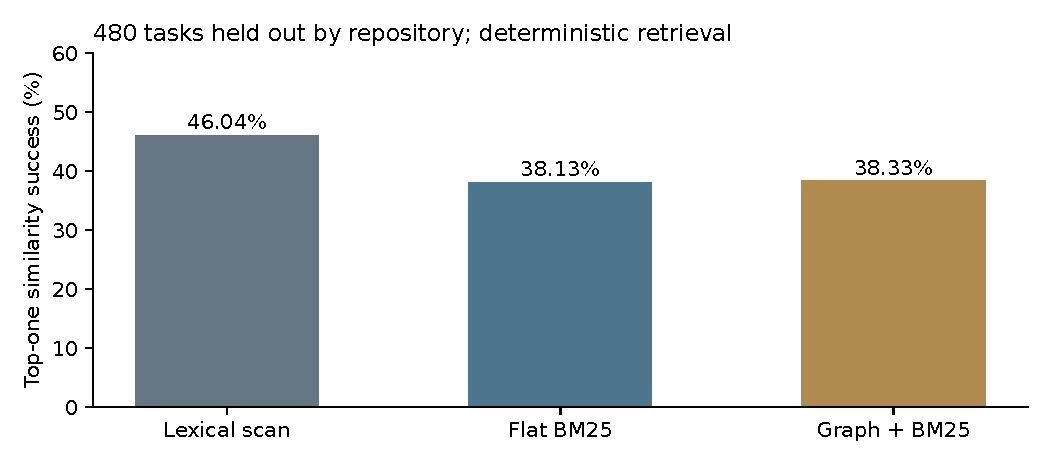
\includegraphics[width=.9\linewidth]{evaluation/figures/success.pdf}\caption{Held-out task proportions. The scan control is a deterministic ranker, not a native Codex harness.}\end{figure}

Graph achieves 184/480 successes (38.33\%) against flat retrieval's 183/480 (38.13\%): a net one task. Graph wins 11 paired cases and loses 10. The paired difference is +0.21 percentage points; the exploratory repository-cluster 95\% interval is [-1.67, +1.88] points. The exact McNemar $p$-value is 1.00. This result supplies no convincing evidence of an advantage for the frozen graph mechanism.

Graph trails scan by 7.71 points. Graph query CPU is 1.76 times flat query CPU, while mean build CPU is about 3.2\% higher. Flat and graph are faster than scanning per query, but that saving comes with lower observed accuracy. Accuracy, latency and construction cost must be reported together.

The entire three-arm assay took about 79 seconds in this container. That aggregate includes extraction, ranking and scoring, but excludes model inference because no model was used. Provider cost and agent repair effect are unmeasured, not zero.


\subsection{Paired uncertainty and transport evidence}
\begin{figure}[ht]\centering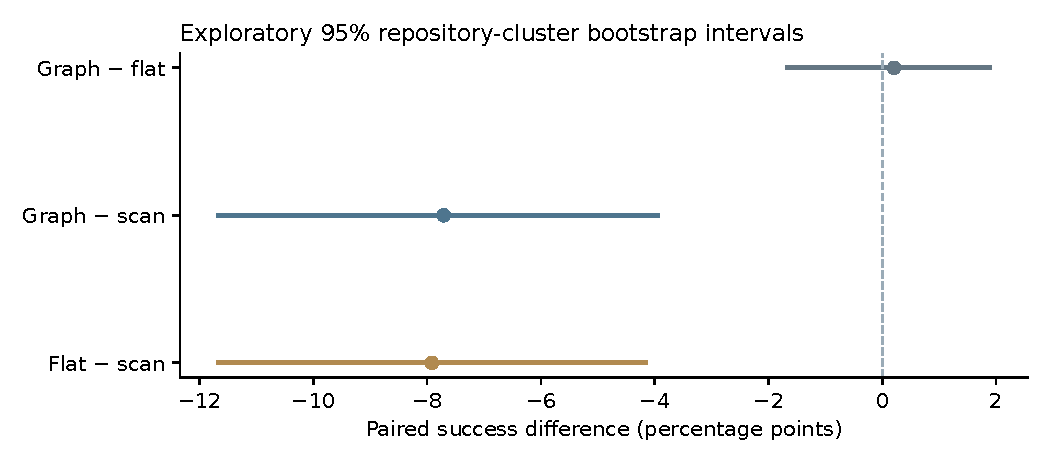
\includegraphics[width=.9\linewidth]{evaluation/figures/differences.pdf}\caption{Exploratory paired differences and 95\% repository-cluster bootstrap intervals, 10,000 draws. They do not estimate a language-model repair effect.}\end{figure}
The six-language MCP audit completed twelve actual query calls: flat and graph, one development repository per language. Every server saw the same source snapshot as the permitted corpus, and discovery/query calls passed. The mean client lifecycle including server startup was about 2.02 seconds across those probes; this does not belong inside the millisecond in-process assay timing. Fixture tests additionally exercise source retrieval, invalid arguments, stale revision, forged IDs and path/response bounds.

The development split scored 42.50\% scan, 45.83\% flat and 44.17\% graph. It contains 120 cases and was not used to select a winning weight configuration. All 480 evaluation targets were extractable under the canonical diagnostic; one development target was not. Per-language outcomes and parse/timing records are published rather than used to select a favourable subgroup.

\subsection{Result and scientific disposition}
This engine is operational as a local evidence service. Its frozen structural reranking did not show a convincing advantage over flat BM25 and was less accurate than a simpler lexical scan in the observed held-out repository population. It consumed more query CPU than flat retrieval. The sensible action is to preserve that result, revise the proposed mechanism under a new development protocol, and keep agent-effectiveness claims behind the unpassed isolation, authentication and accounting gates.

The paper's final result is therefore bounded: a working MCP plus a reproducible, real-data near-null/negative retrieval study. Whether an agent following richer, task-relative abstractions makes better software decisions remains an open empirical question.
\end{document}
